\documentclass[]{article}
\usepackage{lmodern}
\usepackage{amssymb,amsmath}
\usepackage{ifxetex,ifluatex}
\usepackage{fixltx2e} % provides \textsubscript
\ifnum 0\ifxetex 1\fi\ifluatex 1\fi=0 % if pdftex
  \usepackage[T1]{fontenc}
  \usepackage[utf8]{inputenc}
\else % if luatex or xelatex
  \ifxetex
    \usepackage{mathspec}
  \else
    \usepackage{fontspec}
  \fi
  \defaultfontfeatures{Ligatures=TeX,Scale=MatchLowercase}
\fi
% use upquote if available, for straight quotes in verbatim environments
\IfFileExists{upquote.sty}{\usepackage{upquote}}{}
% use microtype if available
\IfFileExists{microtype.sty}{%
\usepackage[]{microtype}
\UseMicrotypeSet[protrusion]{basicmath} % disable protrusion for tt fonts
}{}
\PassOptionsToPackage{hyphens}{url} % url is loaded by hyperref
\usepackage[unicode=true]{hyperref}
\hypersetup{
            pdfborder={0 0 0},
            breaklinks=true}
\urlstyle{same}  % don't use monospace font for urls
\usepackage{graphicx,grffile}
\makeatletter
\def\maxwidth{\ifdim\Gin@nat@width>\linewidth\linewidth\else\Gin@nat@width\fi}
\def\maxheight{\ifdim\Gin@nat@height>\textheight\textheight\else\Gin@nat@height\fi}
\makeatother
% Scale images if necessary, so that they will not overflow the page
% margins by default, and it is still possible to overwrite the defaults
% using explicit options in \includegraphics[width, height, ...]{}
\setkeys{Gin}{width=\maxwidth,height=\maxheight,keepaspectratio}
\IfFileExists{parskip.sty}{%
\usepackage{parskip}
}{% else
\setlength{\parindent}{0pt}
\setlength{\parskip}{6pt plus 2pt minus 1pt}
}
\setlength{\emergencystretch}{3em}  % prevent overfull lines
\providecommand{\tightlist}{%
  \setlength{\itemsep}{0pt}\setlength{\parskip}{0pt}}
\setcounter{secnumdepth}{0}
% Redefines (sub)paragraphs to behave more like sections
\ifx\paragraph\undefined\else
\let\oldparagraph\paragraph
\renewcommand{\paragraph}[1]{\oldparagraph{#1}\mbox{}}
\fi
\ifx\subparagraph\undefined\else
\let\oldsubparagraph\subparagraph
\renewcommand{\subparagraph}[1]{\oldsubparagraph{#1}\mbox{}}
\fi

% set default figure placement to htbp
\makeatletter
\def\fps@figure{htbp}
\makeatother


\date{}

\begin{document}

\section{Lecture 2}\label{header-n0}

\subsection{2.1, 2.2}\label{header-n2}

\subsection{1. 極限 (Limit) 的定義}\label{header-n3}

\begin{itemize}
\item
  用圖例說明\textbf{極限}、\textbf{左極限}和\textbf{右極限},極限的意義從研究一個問題(函數)開始。
  We begin to study the limit by looking at some function:
  \(f\left( x\right) =x^{2}\) Question: What happens to \(f(x)\) when
  \(x\) get to close \(2\) ? (口語:當 \(x\) 靠近 \(2\) 的時後,\(f(x)\)
  會怎麼樣?)
\end{itemize}

\paragraph{\texorpdfstring{\(Def:\)
將此問題記成:}{Def: 將此問題記成:}}\label{header-n11}

\[\lim _{x\rightarrow 2}f\left( x\right)\]

這個問題是一個極限的問題,\(Limit\) (極限),對函數考慮極限,當自變數
\(x\) 靠近 \(2\) 時,對\(f(x)\)的考慮是? 如何用將口語和數學銜接?
把口語寫成一個式子,這個式子代表這個問題:

\[\lim _{x\rightarrow c}g\left( x\right):  當 x 靠近 c 的時後,g(x) 會變成怎麼樣?\]

極限本身是一個式子,是一個事情、一個現象。研究這個答案我們從圖形看起,先從概念開始。

\begin{itemize}
\item
  \textbf{第一個圖形:}

  \[f(x) = x^2\]

  \begin{figure}
  \centering
  \includegraphics{D:/Data/CNotebook/微積分/圖片檔/desmos-graph1.png}
  \caption{}
  \end{figure}
\item
  當 \(x\) 走到2時,有兩種走法:

  \begin{enumerate}
  \def\labelenumi{\arabic{enumi}.}
  \item
    從2的右邊走到2 \((x→2+)\)
  \item
    從2的左邊走到2 \((x→2-)\)
  \end{enumerate}

  其函數值 \(f(x)\) 會趨近4。
\end{itemize}

\[趨近 4 的意思: 跟 4 要多有靠近就有多靠近,趨近是一個概念。\]

\begin{center}\rule{0.5\linewidth}{\linethickness}\end{center}

\subsection{2. 用圖例說明極限、左極限和右極限}\label{header-n40}

\paragraph{\texorpdfstring{\(Def:\) 將此問題與此答案 (其函數值 \(f(x)\)
跟 \(4\) 有多靠近,是走出來的),記成
:}{Def: 將此問題與此答案 (其函數值 f(x) 跟 4 有多靠近,是走出來的),記成 :}}\label{header-n41}

\[\lim _{x\rightarrow 4}f\left( x\right)\]

\(\lim _{x\rightarrow \sqrt {3}}f\left( x\right) =-\sqrt {5}\),這是一個永不停止現象,跟\(-\sqrt {5}\)
要有多靠近就有多靠近,它永遠不會走到這個數,卻跟這個數不可分離。

\begin{center}\rule{0.5\linewidth}{\linethickness}\end{center}

\begin{itemize}
\item
  \textbf{第二個圖形},圖形不包含 \((2,4)\),在 \(x=2\)
  沒有定義,換句話說此函數只定義在不等於 \(2\) :
  \includegraphics{D:/Data/CNotebook/微積分/Calculus_note_1/pics/desmos-graph1.png}
\item
  什麼叫函數 \((function)\)? 構成函數的三大要素:
\item
  \begin{enumerate}
  \def\labelenumi{\arabic{enumi}.}
  \item
    \textbf{定義域 \(x\)}
  \item
    \textbf{對應域 \(f(x)\)}
  \item
    \textbf{如何對應}
  \end{enumerate}

  定義域上的每一個點,在對應域可以找到一個點與它對應。 \(f:A→B \)
  \( by\) \(  f(x)=\) ?

  \( f(x)\) 是函數值、\(f(x)\) 的集合是值域。 
\end{itemize}

Q: \(lim _{x\rightarrow  {2}}f(x)= \) ? A:
\(lim _{x\rightarrow  {2}}f(x)= 4\)
為什麼這兩個圖形不一樣,答案一樣?原因是,是問 \(x\) 逼到
\(2\),它從來不會走到,拿掉 \(x=2\) 沒關係。
討論\(x→2\)的極限時與函數在該點\(x=2\)時,有無定義無關。函數在\(2\)沒有定義,還是可以問
\(lim _{x\rightarrow  {2}}f(x)=\)?

\begin{center}\rule{0.5\linewidth}{\linethickness}\end{center}

\begin{itemize}
\item
  \textbf{第三個圖形} 請問這個圖形在講什麼?在 \(x=2\) 時,定義成 \(8\)
  :

  \begin{figure}
  \centering
  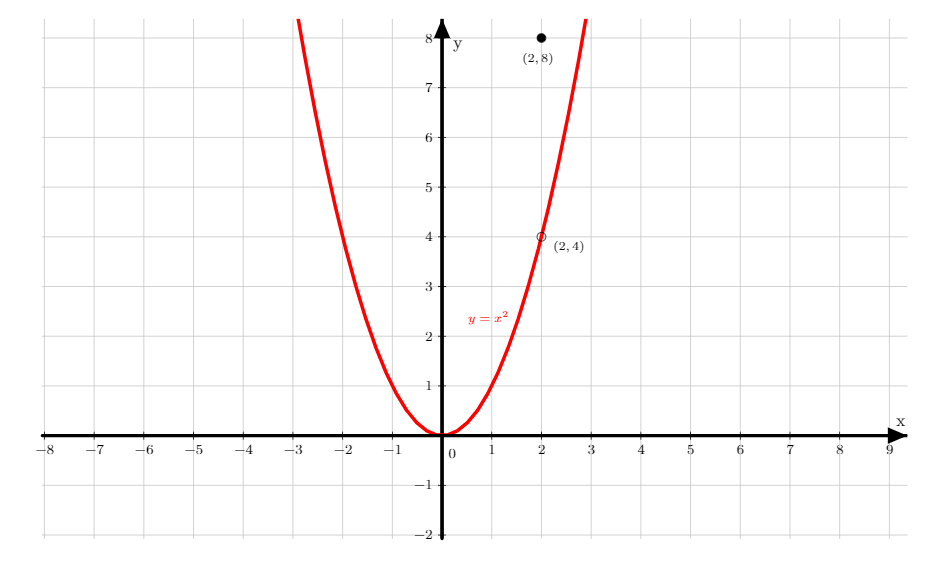
\includegraphics{D:/Data/CNotebook/微積分/Calculus_note_1/pics/下載 (1).png}
  \caption{}
  \end{figure}
\end{itemize}

Q: \(lim _{x\rightarrow  {2}}f(x)= \) ? A:
\(lim _{x\rightarrow  {2}}f(x)= 4\)

\textbf{因為你是問 \(x\) 趨近 \(2\),所以它的極限值跟在 \(x=2\)
的函數值無關。}

\begin{center}\rule{0.5\linewidth}{\linethickness}\end{center}

\begin{itemize}
\item
  \textbf{第四個圖形}

  \begin{figure}
  \centering
  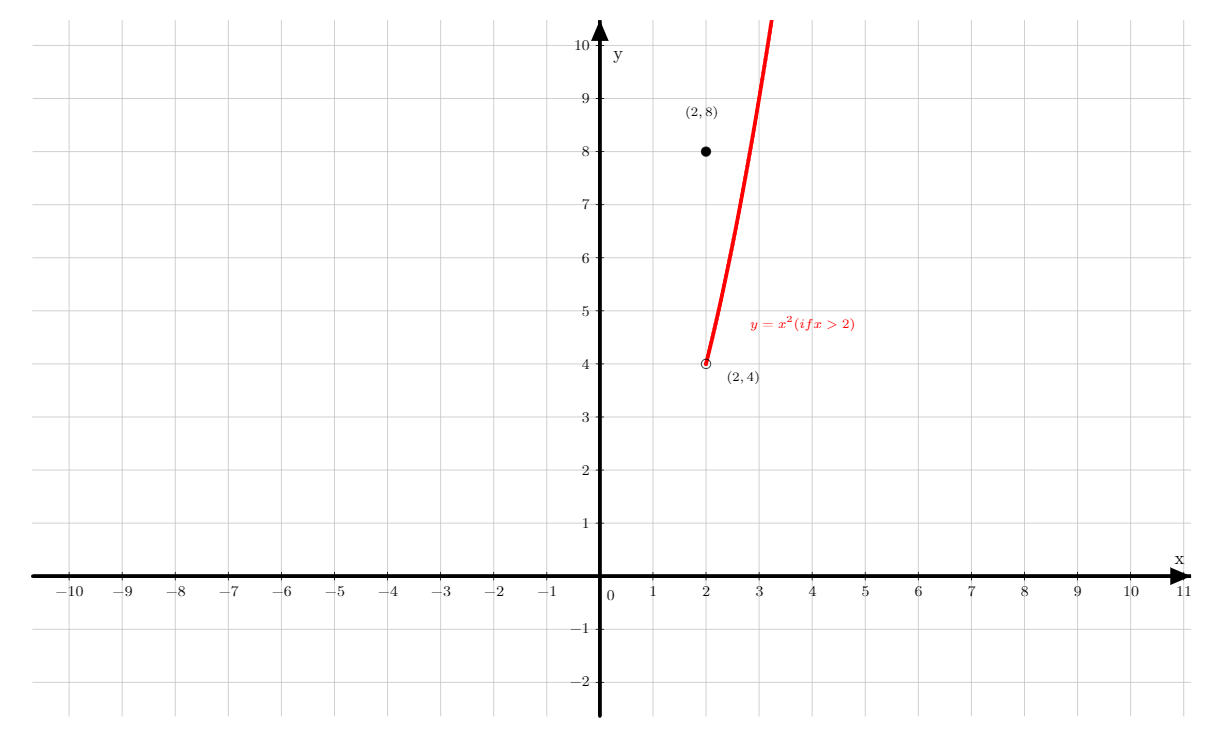
\includegraphics{D:/Data/CNotebook/微積分/Calculus_note_1/pics/下載 (2).png}
  \caption{}
  \end{figure}
\end{itemize}

Q: \(lim _{x\rightarrow  {2}}f(x)= \) ? A: 不存在

因為逼近有兩種,左邊沒有辦法逼近 \(2\)。因為 \(x\) 不能逼近 \(2\) (因為
\(f\) 在 \(x<2\) 時無定義),所以問題不成立→答案不存在 (The limit does't
exist) 。\textbf{左極限與右極限都存在,極限才存在}。

\begin{center}\rule{0.5\linewidth}{\linethickness}\end{center}

\begin{itemize}
\item
  遠離 \(2\) 遠端的函數值變化,不會影響在 \(x=2\)
  附近的變化。(極限值與遠離 \(x=2\) 的情形無關)。
\item
  \textbf{第五個圖形} 當 \(x\) 靠近 \(2\)
  時,會發生無窮大,此問題可以問,因為是問 \(x\) 逼到 \(2\)
  時會發生什麼事:

  \begin{figure}
  \centering
  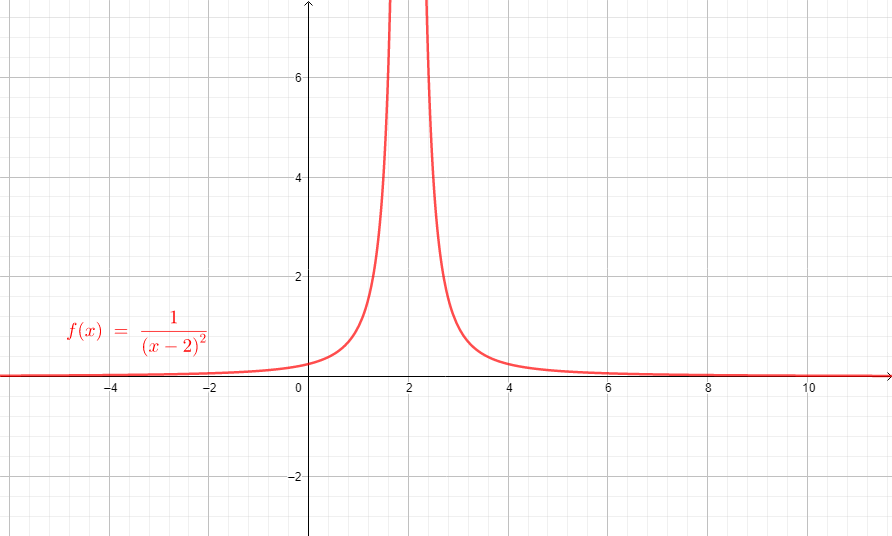
\includegraphics{D:/Data/CNotebook/微積分/Calculus_note_1/pics/try3.png}
  \caption{}
  \end{figure}
\end{itemize}

Q: \(lim _{x\rightarrow  {2}}f(x)= \) ? A: 不存在

此問題可以問,參考例題2。因為你從圖形上觀察到一個現象,函數值要多大有多大,停不下來,沒辦法逼近某值,\textbf{極限值必須是一個定數}。

\begin{center}\rule{0.5\linewidth}{\linethickness}\end{center}

\begin{itemize}
\item
  \textbf{第六個圖形}

  \begin{figure}
  \centering
  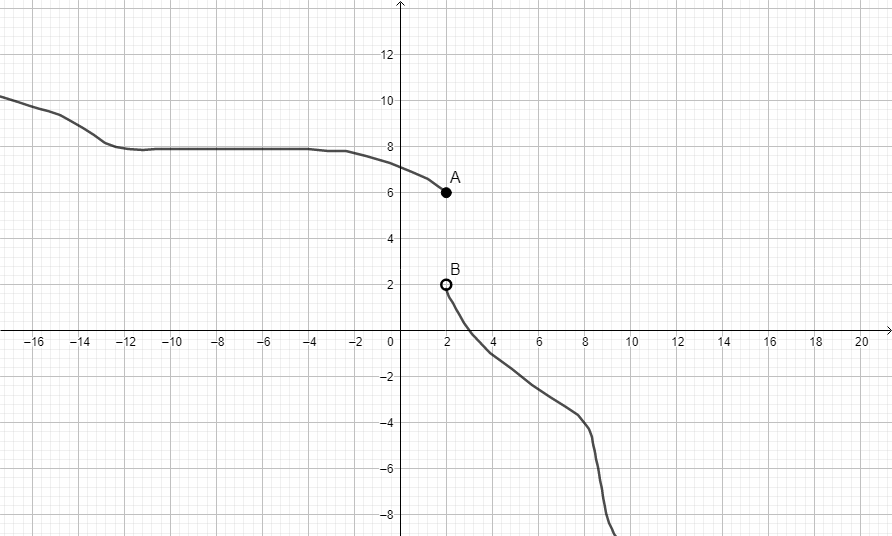
\includegraphics{D:/Data/CNotebook/微積分/Calculus_note_1/pics/try4.png}
  \caption{}
  \end{figure}
\end{itemize}

Q: \(lim _{x\rightarrow  {2}}f(x)= \) ? A: 不存在

因為從左邊逼近 \(6\),從右邊逼近
\(2\),總而言之沒辦法逼到某一個數,左邊逼近不等於右邊逼近。
\textbf{因為x→2-的結果與x→2+的結果不一樣,所以極限不存在。}

\begin{center}\rule{0.5\linewidth}{\linethickness}\end{center}

\begin{itemize}
\item
  \textbf{第七個圖形}
\end{itemize}

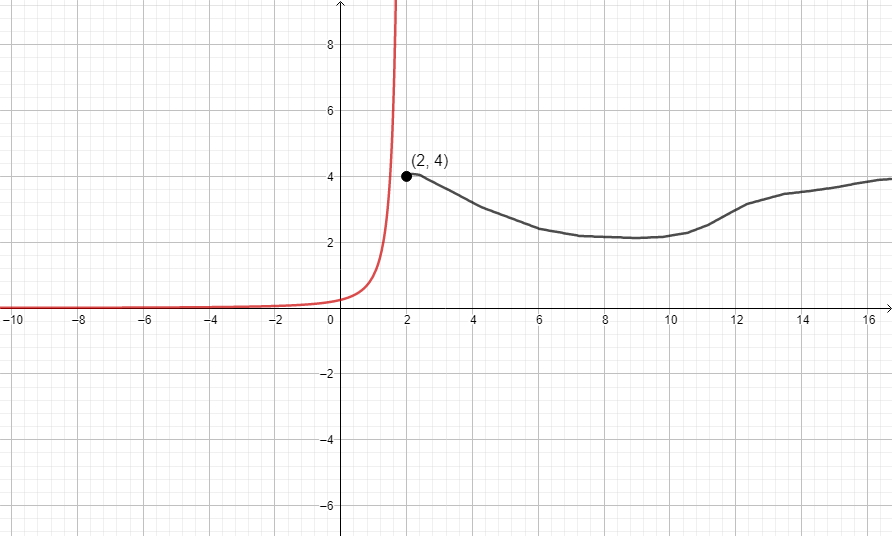
\includegraphics{D:/Data/CNotebook/微積分/Calculus_note_1/pics/try3 (1).png}

Q: \(lim _{x\rightarrow  {2}}f(x)= \) ? A: 不存在
左極限不存在,只要有一邊不存在,則極限就不存在。

\begin{center}\rule{0.5\linewidth}{\linethickness}\end{center}

\begin{itemize}
\item
  e.g. 1

  Calculate \(\lim _{x\rightarrow c}\left| x\right| =\)?

  by drawing the graph

  A: \(|c|\) \(|x|= x\) as \(x>=0\) , \(-x\) as \(x<0\)

  \begin{figure}
  \centering
  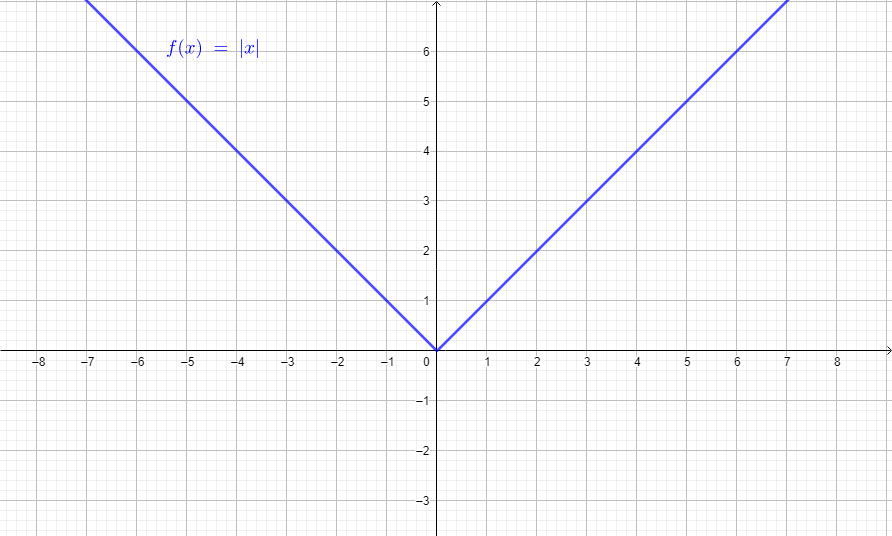
\includegraphics{D:/Data/CNotebook/微積分/Calculus_note_1/pics/geogebra-export.png}
  \caption{}
  \end{figure}
\end{itemize}

\begin{itemize}
\item
  e.g. 2

  \(\lim _{x\rightarrow 0}\dfrac {\left| x\right| }{x}\) ? (By picture!)

  A: 不存在,Therefore 極限不存在(The limit does't exist)
  \(\dfrac {\left| x\right| }{x}\) : \(x=1\) as \(x>0\) 因為分母為 \(0\)
  沒有定義, \(-1\) as \(x<0\)

  \begin{figure}
  \centering
  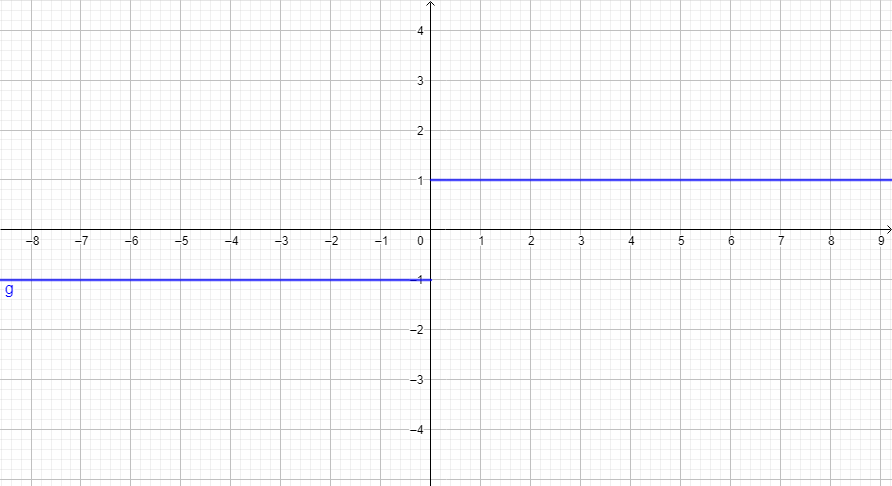
\includegraphics{D:/Data/CNotebook/微積分/Calculus_note_1/pics/geogebra-export (1).png}
  \caption{}
  \end{figure}
\end{itemize}

\begin{center}\rule{0.5\linewidth}{\linethickness}\end{center}

\(Def:\) \(\lim _{x\rightarrow 2+}f\left( x\right) \) 叫做右極限: 當
\(x\) 從右邊逼近 \(2\) 時,\(f(x)\) 會怎麼樣?
\(\lim _{x\rightarrow 2-}f\left( x\right) \) 叫做左極限: 當 \(x\)
從左邊逼近 \(2\) 時,\(f(x)\) 會怎麼樣? \textbf{如果極限存在 ⇔
右極限存在,左極限存在,且相等}。

Next time: 極限真正困難是: 如果我不會畫圖,我該如何得到極限值?

\end{document}
